% バックエンドの話も一部ここに持ってこよう
\section{組織内コミュニケーションツールでの投票}
本システムでは，研究室内で使用されているチャットツールであるSlackを採用し，SlackBotを用いてダイレクトメッセージ(以下DM)の送信および投票の受付を実現した．
%

% 帰宅推奨時刻の算出時に抽出した最多区間内のメンバに時刻情報を含んだダイレクトメッセージを送信し投票を促す．
% これによりユーザ側から近しい時刻に帰りそうな具体的なメンバを分からない状態にし，メンバ以外へのコミュニケーションの発生も狙った．

最多区間内に含まれるユーザは，帰宅推奨時刻付近で帰宅する可能性が高いと考えられる．
そのため，本システムでは，これらのユーザを帰宅同行の中心的な候補として位置付け，Slackを用いたDMの送信対象としている．
これにより，帰宅同行の可能性が低いユーザへの不要な通知を避けつつ，実際に同行が成立しやすいユーザに対して重点的にアプローチできる設計としている．

DMでは，「乗れそうなバスを選択してください」という文言とともに，算出されたバスの時刻を番号付きの選択肢として提示する．
\begin{figure}[htb]
  \centering
  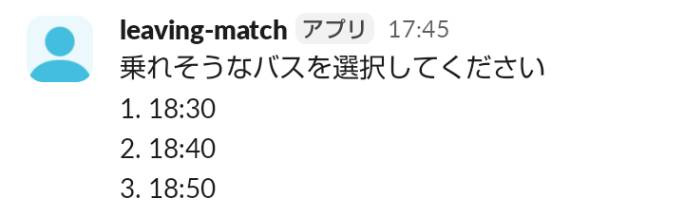
\includegraphics[width=0.6\linewidth]{slack.jpg} % suzuki
  \caption{SlackBotとのDMのスクリーンショット}
  \label{fig:slack}

\end{figure}

例えば三択の場合には，
\begin{description}
  \itemindent=1zw
  \itemsep=0mm
  \parsep=0mm
  \item 1. 19:30
  \item 2. 19:45
  \item 3. 20:00
\end{description}
のように表示され，二択の場合には
\begin{description}
  \itemindent=1zw
  \itemsep=0mm
  \parsep=0mm
  \item 1. 19:45
  \item 2. 20:00
\end{description}
のように提示される．
選択肢数に応じて表示を自動的に切り替え，ユーザは常に同じ操作感で投票を行える．
%同一ユーザの複数投票の扱い 投票変更可

また，投票は$1\sim$3の数字を入力させ打ち間違いを減らし，ユーザの手間を減らす設計にした．
複数の時刻への投票を可能とし，帰宅時刻を柔軟に変更できるユーザがより投票しやすい設計にした．
同一ユーザによる複数回の投票が行われた場合には，最新の投票内容のみを有効とする．


DMの送信および投票受付は，三択の時刻が算出された時点で開始され，最多投票の時刻が決定するまでの間に行われた投票のみを集計対象とする．
この時間帯以外に送信されたメッセージは集計されない．
なお，投票の受付から集計までの一連の処理は，すべてユーザとSlackBotとの個別DM内で完結する設計としている．
これによりユーザ側から近しい時刻に帰りそうな具体的なメンバを分からない状態にし，メンバ以外へのコミュニケーションの発生も狙った．
